\documentclass{article}
\usepackage{tikz, comment}
\usepackage{pifont}
\usepackage{fontspec, pgfplots}
\usetikzlibrary{arrows, decorations.markings, decorations.pathreplacing}
\begin{comment}
:Title: Not defined yet
:Tags: moment;area using parametric equations,parametric integral formula;apothem;focus of a parabola;directrix of a parabola
:Prob: 0.6232;0.6159;0.6029;0.6018;0.5991
:Author: Prof.Hu Ji-shan, HKUST
:Slug: No name yet

Description Here.........
\end{comment}
\begin{document}\centering 

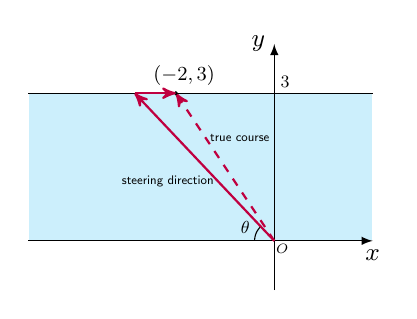
\begin{tikzpicture}[>=latex,xscale=.5*1.25, yscale=.5*1.25][font=\sf\small] 

\draw[white, fill=cyan!20] (-5, 0)--++(7, 0)--++(0, 3)--++(-7, 0)--cycle;  

\draw[->] (-5, 0) -- (2, 0)node[below] {$x$} ;
\draw[->] (0, -1) -- (0, 4)node[left] {$y$} ;

\draw (-5, 3) -- (2, 3);

\draw [dashed, purple, thick, ->, >=stealth'](0, 0) -- (-2, 3) node[black, above, xshift=3, scale=0.8]{$(-2,3)$}node[black, right, midway, pos=0.7, xshift=0, yshift=0, scale=0.5]{true course};

\draw[fill] (-2,3) circle(0.03);

\draw [purple, thick, ->, >=stealth'](0, 0) -- ({-3*tan(43.4)}, 3)node[black, left, midway, pos=0.4, xshift=0, yshift=0, scale=0.5]{steering direction};
\draw [purple, thick, ->, >=stealth']({-3*tan(43.4)}, 3)--(-2,3);

\node[right, yshift=4, scale=0.7] at (0, 3) {$3$};

\draw[black, samples=100, smooth, domain=136.6:180, variable=\t] 
		plot ({0.4*cos(\t)}, {0.4*sin(\t)}); 

\node[left, yshift=2, scale=0.7] at ({0.4*cos(158)}, {0.4*sin(158)}) {$\theta$};

\node[scale=0.7] at (0.2/1.25, -0.2/1.25) {\scriptsize$O$};

\end{tikzpicture}
\end{document}